\documentclass[11pt]{article}

\usepackage[a4paper,margin=1in]{geometry}
\usepackage{amsmath,amssymb,amsfonts,amsthm,mathtools}
\usepackage{bm}
\usepackage{graphicx}
\usepackage{booktabs}
\usepackage{caption}
\usepackage{hyperref}
\usepackage{enumitem}
\usepackage{microtype}
\usepackage{cleveref}

\numberwithin{equation}{section}
\newtheorem{proposition}{Proposition}[section]
\newtheorem{lemma}[proposition]{Lemma}
\theoremstyle{remark}
\newtheorem{remark}[proposition]{Remark}

\newcommand{\R}{\mathbb{R}}
\newcommand{\Dm}{\mathsf{D}}
\newcommand{\K}{\mathsf{K}}
\newcommand{\capp}{c_{\mathrm{app}}}
\newcommand{\figB}{test_plots/dmp}
\newcommand{\figC}{test_plots/direction_C_nonfourier_phase_change/flux_audit}
\newcommand{\figA}{test_plots/benchmark/external_codes}

\title{Bound Preservation with Sign-Changing Sources, Consistent Dirichlet\\
Boundary Fluxes, and Cross-Code Validation in Thermalio}
\author{Thermalio research notes --- follow-up to Directions A, B and C}
\date{}

\begin{document}
\maketitle

\begin{abstract}
We close three open items of the Thermalio research backlog.
\textbf{(B)} The global maximum-principle limiter of the algebraic flux
correction (AFC) scheme used bounds detected from initial and boundary data,
which are invalid once a source of either sign moves the solution outside that
range.  We add a \emph{source envelope} limiter whose time-dependent bounds are
proved by a discrete comparison principle, and a \emph{source-local} limiter
whose bounds come from the source-including low-order solution.  The envelope
limiter is exactly as accurate as the unlimited high-order scheme (relative
error $2.38\times10^{-4}$ vs.\ $4.60\times10^{-3}$ for the previous limiter) and
never leaves the rigorous bounds, which the high-order scheme violates by $0.063$.
\textbf{(C)} We reconstruct the heat flowing through Dirichlet boundaries as
the residual of the constrained boundary-cell equations.  This makes the
energy audits of the cryosurgery and quench scenarios \emph{non-tautological}:
the previous audits inferred the boundary energy from the enthalpy change and
were zero by construction; the new audits show closure errors of $26\%$ and
$32\%$ on a $24$-cell mesh, which we decompose exactly into a latent-heat jump in
the Dirichlet band ($L\times$ band area), an interior apparent-capacity defect
that vanishes with $\Delta t$, and unconverged Picard residuals.  The enthalpy
solver closes to $10^{-16}$.
\textbf{(A)} We validate Thermalio against two independent external codes,
FiPy~4.0.3 (finite volumes) and scikit-fem~12.0.2 (P1/P2 finite elements), on
isotropic, anisotropic and Robin/Pennes manufactured problems, and the enthalpy
solver against Neumann's classical Stefan solution.  All codes agree and
converge at their nominal rates on isotropic problems.  On the anisotropic
problem, Thermalio's reconstructed flux stays near second order while FiPy's
tensor diffusion drops to order $0.6$--$0.9$.  The study also exposed a
limitation of Thermalio itself: on skewed meshes the anisotropic case fell to
about first order.
\textbf{(B$'$)} We trace that loss to the \texttt{reconstructed} flux (averaged
linearly exact gradients, no compact coupling).  We replace it with a new
\emph{quadratic} flux: a 2-exact least-squares reconstruction from cell
averages, face-midpoint gradients and a consistent compact jump penalty.  The
new flux reproduces quadratic solutions to $10^{-14}$ on every mesh tested and
restores second order on skewed ($2.00$), hexagonal ($1.93$), randomly perturbed
($2.03$) and tiled mixed-polygon ($1.92$) meshes.  On the last three, every
previous option stalls at order $0.2$--$1.1$.
\end{abstract}

\tableofcontents

%=============================================================================
\section{Bound preservation with sign-changing sources (Direction B, PR5)}
%=============================================================================

\subsection{Setting and the AFC scheme}

For $u_t-\nabla\cdot(\bm K\nabla u)=q$ with Dirichlet data $g$, the high-order
FV operator $\mathsf A_H$ (reconstructed or non-orthogonally corrected flux) is
consistent but not an M-matrix.  Thermalio's AFC solver (PRs 2--4) uses the
low-order operator $\mathsf A_L=\mathsf A_H+\mathsf D$, with
$d_{ij}=-\max(0,a_{ij},a_{ji})$ off the diagonal and zero row sums, which is an
M-matrix with zero row sums.  The difference is written as antisymmetric edge
fluxes $f_{ij}=d_{ij}(u_i-u_j)$.  One backward-Euler step solves
\begin{equation}
  (\Dm+\Delta t\,\mathsf A_L)u^{n+1}
  = \Dm(u^n+\Delta t\,q^{n+1}) + \Delta t\sum_j \alpha_{ij}f_{ij}(u^{n+1}),
  \qquad \text{identity rows on Dirichlet cells},
  \label{eq:afc}
\end{equation}
with Zalesak limiter coefficients $\alpha_{ij}\in[0,1]$ chosen so that the
anti-diffusive correction keeps each node inside bounds
$[u_i^{\min},u_i^{\max}]$ ($\alpha\equiv0$ gives the low-order solution
$u^L$; $\alpha\equiv1$ gives the high-order one).  The scheme's properties
are therefore determined by the bounds.

\paragraph{Why the PR4 global limiter fails with sources.}  PR4 sets
$u^{\min}\equiv m$, $u^{\max}\equiv M$, where $m$ and $M$ are the extrema of the
initial and boundary data.  This is rigorous only if the continuous problem
obeys $m\le u\le M$, i.e.\ for $q\equiv0$ or sign-definite $q$.  With a
sign-changing source the true solution leaves $[m,M]$.  Wherever the low-order
solution exceeds $M$, the Zalesak capacity $Q_i^+\propto\max(M-u_i,0)$ is
zero, so the correction is switched off there and the scheme falls back to the
low-order (inconsistent on skewed meshes) operator.

\subsection{The source envelope}

\begin{proposition}[Discrete comparison envelope]
\label{prop:envelope}
Let $\mathsf A_L$ be an M-matrix with zero row sums and $\Dm>0$ diagonal.
Define $M^0=\max(\max_iu^0_i,\max g^0)$, $m^0=\min(\min_iu^0_i,\min g^0)$ and
\begin{equation}
\begin{aligned}
  M^{n+1}&=\max\Big(M^n+\Delta t\max_{i\in\mathcal I}(q_i^{n+1})^+,\ \max g^{n+1}\Big),\\
  m^{n+1}&=\min\Big(m^n-\Delta t\max_{i\in\mathcal I}(q_i^{n+1})^-,\ \min g^{n+1}\Big).
\end{aligned}
  \label{eq:envelope}
\end{equation}
If $m^n\le u^n\le M^n$, then the low-order solution satisfies
$m^{n+1}\le u^{L}\le M^{n+1}$.
\end{proposition}
\begin{proof}
Let $v\equiv M^{n+1}$ (a constant vector).  Because the row sums are zero,
$(\Dm+\Delta t\mathsf A_L)v=\Dm v$.  On interior rows,
$|\Omega_i|M^{n+1}\ge|\Omega_i|(M^n+\Delta t\,q_i^{n+1})\ge|\Omega_i|(u_i^n+\Delta t\,q_i^{n+1})$.
On Dirichlet rows, $v_i=M^{n+1}\ge g_i$.  So $v$ is a discrete supersolution,
and the system matrix with identity Dirichlet rows is inverse-nonnegative
(M-matrix), which gives $u^L\le v$.  The lower bound is symmetric.
\end{proof}

The continuous analogue holds too: $w(t)=M^0+\int_0^t\max_xq^+\,\mathrm ds$
satisfies $w_t\ge q$ and $w\ge g$, so $u\le w$ by the parabolic comparison
principle.  The \texttt{source\_envelope} limiter enforces
$u^{\min}\equiv m^{n+1}$, $u^{\max}\equiv M^{n+1}$ in \eqref{eq:afc}.
\begin{itemize}[leftmargin=*]
\item It never clips the true solution, because the true solution satisfies
  the same type of bound.
\item It does not clip smooth interior extrema, which lie inside the envelope.
  This is the mechanism that gave PR4 its accuracy.
\item For $q\equiv0$ it reduces to PR4 exactly (verified to $10^{-13}$ in the unit tests).
\end{itemize}

\subsection{Source-local bounds}

\begin{lemma}[Local convex-combination property of the low-order step]
On an interior row with $\ell_{ij}=-(\mathsf A_L)_{ij}\ge0$, the low-order
solution satisfies
\[
  u^L_i=\frac{|\Omega_i|\,\tilde u_i+\Delta t\sum_j\ell_{ij}u^L_j}{|\Omega_i|+\Delta t\sum_j\ell_{ij}},
  \qquad \tilde u_i=u_i^n+\Delta t\,q_i^{n+1},
\]
a convex combination of the source-advanced old value $\tilde u_i$ and the new
neighbour values.
\end{lemma}
Source-driven extrema are therefore already present in $u^L$.  The
\texttt{source\_local} limiter takes $[u_i^{\min},u_i^{\max}]$ as the range of
$u^L$ over the stencil of $i$.  The high-order correction may then sharpen
features but not create extrema beyond those the monotone, source-including
scheme produces.  Since $u^L$ lies inside the envelope
(\cref{prop:envelope}), these bounds are at least as strict.  As with all
local limiters, smooth extrema are clipped unless the smoothness relaxation of
PR3 is enabled; the relaxed variant is not strictly bound-preserving.

\subsection{Results}

\begin{figure}[h]
\centering
\includegraphics[width=\textwidth]{\figB/sign_changing_sources.png}
\caption{(a) Manufactured solution $u=(0.2+4t)\sin\pi x\sin\pi y$ under a
sign-changing source.  It grows from $[-0.2,0.2]$ to $[-0.4,0.4]$, outside the
data range.  Anisotropic tensor (ratio 5, $30^\circ$), skewed mesh.
(b) Excess over the rigorous envelope for a steep block with a heater and a
sink (ratio 20).  (c) Maximum violation and error against a fine-mesh reference.
(d) Where the high-order scheme leaves the envelope: at block corners aligned
with the anisotropy.}
\label{fig:B}
\end{figure}

\begin{table}[h]
\centering
\caption{Relative $L^2$ error for the growing manufactured solution (\cref{fig:B}a).}
\begin{tabular}{@{}lcccc@{}}
\toprule
scheme & $n=12$ & $24$ & $48$ & $96$ \\
\midrule
high-order (unlimited) & $5.48\mathrm{e}{-3}$ & $2.09\mathrm{e}{-3}$ & $7.72\mathrm{e}{-4}$ & $2.38\mathrm{e}{-4}$ \\
low-order M-matrix & $6.75\mathrm{e}{-3}$ & $8.22\mathrm{e}{-3}$ & $8.28\mathrm{e}{-3}$ & $7.87\mathrm{e}{-3}$ \\
PR4 global (auto bounds) & $5.56\mathrm{e}{-3}$ & $4.38\mathrm{e}{-3}$ & $4.51\mathrm{e}{-3}$ & $4.60\mathrm{e}{-3}$ \\
\textbf{source envelope} & $5.48\mathrm{e}{-3}$ & $2.09\mathrm{e}{-3}$ & $7.72\mathrm{e}{-4}$ & $2.38\mathrm{e}{-4}$ \\
source local, strict & $6.93\mathrm{e}{-3}$ & $4.12\mathrm{e}{-3}$ & $2.74\mathrm{e}{-3}$ & $4.21\mathrm{e}{-3}$ \\
source local, relaxed & $5.48\mathrm{e}{-3}$ & $2.09\mathrm{e}{-3}$ & $7.72\mathrm{e}{-4}$ & $1.19\mathrm{e}{-3}$ \\
\bottomrule
\end{tabular}
\label{tab:B}
\end{table}

On the steep problem (\cref{fig:B}b--d) the high-order scheme exceeds the
envelope by up to $0.063$, and so does the relaxed local limiter ($0.061$).  The
envelope, strict local, PR4 and low-order schemes stay inside it.  The
sink-driven minimum ($\approx-0.028$ for the envelope limiter) is \emph{not}
clipped.  A fine-mesh high-order reference leaves the envelope by only
$4.6\times10^{-4}$: the violation is a discretization artifact that vanishes
under refinement.  The $L^2$ errors against that reference ($0.14$--$0.18$) are
dominated by the coarse resolution of the discontinuous data and do not
separate the schemes; accuracy is assessed by \cref{tab:B}.

\paragraph{Assessment.}  The envelope limiter is the recommended default for
sign-changing sources.  It is rigorous, as accurate as the unlimited scheme, and
inexpensive.  Its bounds are global and can be loose, so it does not suppress
small \emph{local} oscillations that stay within the envelope.  The strict
local limiter does, at first-order accuracy.

%=============================================================================
\section{Consistent Dirichlet boundary fluxes (Direction C, capability 7)}
%=============================================================================

\subsection{Reaction flux}

Thermalio imposes Dirichlet data by replacing the equations of the boundary-cell
band $\mathcal B$ with $u_i=g_i$, so the heat crossing $\partial\Omega$ is never
computed.  Following the consistent-flux idea of Hughes et al.\ \cite{hughes2000},
we evaluate the \emph{unconstrained} cell balance on $\mathcal B$ at the
computed solution:
\begin{equation}
  r_i^{n+1} = |\Omega_i|\,\mathcal T_i^{n+1} + (\K u^{n+1})_i - |\Omega_i|q_i^{n+1}-b_i^{n+1},
  \qquad i\in\mathcal B,
  \label{eq:reaction}
\end{equation}
where $\mathcal T_i$ is the scheme's own discrete time term (e.g.\
$(H_i^{n+1}-H_i^n)/k$ for the enthalpy solver;
$\tau D^2u+\capp D^1u$ for the apparent-capacity Cattaneo--Stefan solver).
$r_i$ is the heat flow into cell $i$ through $\partial\Omega$ needed to hold
$u_i=g_i$.

\begin{proposition}[Exact global balance]
If the FV operator is conservative (each face flux is added to one cell and
subtracted from its neighbour, so that $\mathbf 1^{\!\top}\mathsf A=0$), then
summing the cell equations gives
\begin{equation}
  \sum_i|\Omega_i|\mathcal T_i^{n+1}=\sum_i|\Omega_i|q_i^{n+1}+\sum_ib_i^{n+1}
  +\sum_{i\in\mathcal B}r_i^{n+1}+\sum_{i\in\mathcal I}\rho_i^{n+1},
\end{equation}
where $\rho_i$ is the residual of interior equations (zero for converged nonlinear solves).
\end{proposition}
Thermalio's TPFA, non-orthogonal and reconstructed operators have
$\mathbf 1^{\!\top}\mathsf A=0$ to round-off; the audit records this.

\subsection{Audit identity for the apparent-capacity Cattaneo--Stefan scheme}

With $D^2u=(u^{n+1}-2u^n+u^{n-1})/\Delta t^2$ and
$D^1u=(u^{n+1}-u^{n-1})/(2\Delta t)$, multiplying by $\Delta t$ and summing over
steps, the relaxation term telescopes:
\begin{equation}
  \underbrace{\tau\sum_i|\Omega_i|\frac{(u^N-u^{N-1})-(u^0-u^{-1})}{\Delta t}}_{\text{relaxation storage }R}
  +\underbrace{\Delta t\sum_n\sum_i|\Omega_i|\capp(u^{n+1})D^1u}_{\text{capacity work }C}
  = Q+F+\varrho,
  \label{eq:identity}
\end{equation}
with source energy $Q$, reconstructed boundary energy
$F=\Delta t\sum_n\sum_{\mathcal B}r^{n+1}$ and unconverged-step residual
$\varrho$.  The enthalpy audit compares the true enthalpy change
$\Delta E=\sum_i|\Omega_i|[H(u^N_i)-H(u^0_i)]$ with $Q+F-R$:
\begin{equation}
  \Delta E-(Q+F-R) = \underbrace{(\Delta E-C)}_{\text{capacity defect}}+\varrho .
\end{equation}
\Cref{eq:identity} holds to $10^{-15}$ in every run (unit test and study).

\begin{lemma}[Latent-heat jump of the Dirichlet band]
\label{lem:band}
If a band cell is initialized at $T_0$ (liquid) while $g$ lies below the
solidus, the cell jumps to $g$ in the first step.  Its true enthalpy change
is $c(g-T_0)-L$, while the apparent-capacity time term (with
$\capp(g)=c$) accounts for only $c(g-T_0)$.  The band's contribution to the
capacity defect is therefore $-L\sum_{i\in\mathcal B_{\mathrm{jump}}}|\Omega_i|$,
independently of $\Delta t$.
\end{lemma}
We therefore also report an \emph{interior} audit, using the band-to-interior
flux $-\sum_{i\in\mathcal I}(\mathsf Au)_i$, which isolates the scheme's own
defect.

\subsection{Results}

\begin{figure}[h]
\centering
\includegraphics[width=\textwidth]{\figC/flux_audit.png}
\caption{(a) Cryosurgery: energy extracted measured two independent ways.
For the enthalpy solver the reconstructed flux and the enthalpy loss coincide;
for the apparent-capacity solver they differ by $26\%$.  (b) Exact
decomposition of the closure residual.  (c) Closure residual vs.\ $\Delta t$:
full domain (band jump, $\Delta t$-independent), interior only (decreasing), enthalpy
solver ($10^{-16}$).  (d) Per-cell reaction flux along the cryoprobe.}
\label{fig:C}
\end{figure}

\begin{table}[h]
\centering
\caption{Audit decomposition, apparent-capacity Cattaneo--Stefan solver, $24$-cell
mesh, $100$ steps (energy units).  Lemma~\ref{lem:band} predicts band jumps
$-L|\mathcal B_{\mathrm{jump}}|=-0.1667$ and $-0.612$.}
\begin{tabular}{@{}lrr@{}}
\toprule
& cryosurgery & quench \\
\midrule
enthalpy change $\Delta E$ & $-0.639$ & $-1.864$ \\
reconstructed boundary energy $F$ & $-0.475$ & $-1.276$ \\
relaxation storage $R$ & $-0.0006$ & $-0.0023$ \\
band latent jump & $-0.1667$ & $-0.612$ \\
interior capacity defect & $+0.085$ & $+0.065$ \\
unconverged-step residual $\varrho$ & $-0.084$ & $-0.043$ \\
\textbf{closure residual} & $-0.165\ (26\%)$ & $-0.590\ (32\%)$ \\
identity \eqref{eq:identity} residual & $<10^{-15}$ & $<10^{-15}$ \\
enthalpy solver closure & $-1.1\times10^{-16}$ & $2.2\times10^{-16}$ \\
\bottomrule
\end{tabular}
\label{tab:C}
\end{table}

As $\Delta t$ decreases from $0.02$ to $0.00125$, the interior capacity defect
for cryosurgery falls from $0.18$ to $0.017$ and the unconverged residual from
$0.23$ to $0.008$, while the band jump stays at $-0.1667$.  The production
application runners (\texttt{direction\_c\_applications.py}) now use this
audit.  At their default $40\times40$ and $36\times18$ resolutions they report
relative closure residuals of $-2.1\%$ (cryosurgery) and $-12.5\%$ (quench),
where the previous inferred audit reported exactly zero.

%=============================================================================
\section{Cross-code validation against external codes (Direction A)}
%=============================================================================

\subsection{Codes and protocol}

\begin{itemize}[leftmargin=*]
\item \textbf{Thermalio}: cell-centred FV (reconstructed flux) on square and
  skewed ($0.3$) quadrilateral meshes.  Dirichlet data are imposed on the
  boundary-cell band at cell centres; Robin data use a one-sided face closure.
\item \textbf{FiPy 4.0.3} \cite{guyer2009}: NIST cell-centred FV on
  \texttt{Grid2D}.  Dirichlet values are imposed on faces; a rank-2 face
  coefficient is used for the tensor; SciPy LU backend.
\item \textbf{scikit-fem 12.0.2} \cite{gustafsson2020}: continuous Galerkin
  P1/P2 on a structured triangulation.  Dirichlet data are imposed nodally,
  Robin data weakly.
\end{itemize}
All codes share no source with Thermalio's solvers (\texttt{heat\_solver/external\_codes.py}
only calls their public APIs) and use backward Euler with the same
$\Delta t=2.5\times10^{-4}$, $t_f=0.05$.  The temporal error ($\approx5\times10^{-6}$)
is therefore common and small.  FV errors are discrete relative $L^2$ norms at
cell centres; FEM errors are exact $L^2$ norms by quadrature.  Cross-code
differences are evaluated at Thermalio's cell centres (FiPy's centres coincide;
FEM solutions are interpolated with \texttt{basis.probes}).

\begin{figure}[h]
\centering
\includegraphics[width=\textwidth]{\figA/external_code_comparison.png}
\caption{(a)--(c) Convergence to the exact solution; legend values are
finest-pair orders.  (d) Code-to-code differences.  (e) Work--precision for
the anisotropic case.  (f) Enthalpy Stefan solver vs.\ Neumann's similarity
solution.}
\label{fig:A}
\end{figure}

\begin{table}[h]
\centering
\caption{Relative $L^2$ error at $n=64$ (finest-pair observed order in brackets).}
\small
\begin{tabular}{@{}lccc@{}}
\toprule
code & isotropic & anisotropic (ratio 5) & Pennes + Robin \\
\midrule
Thermalio, square & $3.30\mathrm{e}{-4}\ (2.05)$ & $3.09\mathrm{e}{-5}\ (1.75)$ & $2.54\mathrm{e}{-5}\ (1.91)$ \\
Thermalio, skewed & -- & $1.41\mathrm{e}{-4}\ (0.88)$ & -- \\
FiPy & $8.34\mathrm{e}{-5}\ (1.92)$ & $5.25\mathrm{e}{-4}\ (0.92)$ & -- \\
scikit-fem P1 & $2.02\mathrm{e}{-3}\ (2.00)$ & $1.93\mathrm{e}{-3}\ (2.00)$ & $1.03\mathrm{e}{-4}\ (2.01)$ \\
scikit-fem P2 & $1.53\mathrm{e}{-5}\ (2.89)$ & $1.54\mathrm{e}{-5}\ (2.88)$ & $5.45\mathrm{e}{-6}$ (time floor) \\
\bottomrule
\end{tabular}
\label{tab:A}
\end{table}

\subsection{Findings}

\begin{enumerate}[leftmargin=*]
\item \textbf{Agreement.}  All codes converge at their nominal orders on the
  isotropic and Robin/Pennes problems.  The Thermalio--FiPy and
  Thermalio--scikit-fem (P2) differences decay at second order to
  $2.5\times10^{-4}$ and $2.5\times10^{-5}$--$3.2\times10^{-4}$.  This is
  independent-code verification of Thermalio's diffusion, Robin and perfusion
  discretizations.
\item \textbf{Error constants.}  On the isotropic problem Thermalio's error is
  $4\times$ FiPy's at equal cell count.  The difference comes from the Dirichlet
  convention: FiPy imposes $g$ on boundary faces, while Thermalio holds the whole
  boundary-cell band at $g(\bm x_i)$, which is still second-order consistent but
  shifts the effective boundary by half a cell.
\item \textbf{Anisotropy.}  With a rotated tensor, Thermalio's reconstructed
  flux stays close to second order (orders $1.85, 1.90, 1.75$) and is $17\times$
  more accurate than FiPy at $n=64$.  FiPy's rank-2 face coefficient on
  \texttt{Grid2D} converges at order $0.6$--$0.9$ in this test.  We report this as
  observed behaviour of the documented API, not as a general statement about FiPy.
\item \textbf{Limitation of Thermalio (now fixed).}  On the skewed mesh the same
  anisotropic problem converged at orders $1.34\to1.07\to0.88$ with the
  \texttt{reconstructed} flux.  \Cref{sec:quadratic} diagnoses the cause and
  introduces the quadratic flux.  In this cross-code protocol it reaches
  $1.45\times10^{-5}$ at $n=64$ (``Thermalio FV quadratic (skewed mesh)'' in
  \cref{fig:A}), $10\times$ below the \texttt{reconstructed} flux
  ($1.41\times10^{-4}$).  Its finest-pair order here ($1.51$) is capped by the
  shared backward-Euler time floor; with Crank--Nicolson it is $2.00$
  (\cref{tab:Q}).
\item \textbf{Time-error floor.}  P2 reaches the common backward-Euler floor of
  $\approx5\times10^{-6}$ on the Robin problem, which is why its last observed order is
  $0.23$.
\item \textbf{Cost.}  At $n=64$ the wall times are: Thermalio $1.6$\,s,
  scikit-fem P1 $3.5$\,s, FiPy $5$--$6$\,s, scikit-fem P2 $34$\,s.  P2 is the
  most accurate per degree of freedom on these smooth problems.
\end{enumerate}

\subsection{Neumann's Stefan problem}

A solid at the melting temperature $T_m=0$ is melted by a wall at $T_w=1$.  With
Stefan number $\mathrm{St}=c(T_w-T_m)/L=0.5$, the front is
$s(t)=2\lambda\sqrt{\alpha t}$, where
$\lambda e^{\lambda^2}\operatorname{erf}\lambda=\mathrm{St}/\sqrt\pi$
($\lambda=0.4648$), and the liquid temperature is
$T=T_w[1-\operatorname{erf}(x/2\sqrt{\alpha t})/\operatorname{erf}\lambda]$
\cite{carslaw1959}.  The enthalpy solver ($\Delta x=1/160$, nearly sharp ramp
of width $10^{-3}$) tracks the front with a maximum error of
$8.2\times10^{-4}=0.13\,\Delta x$ over $t\in[0.02,0.5]$ (\cref{fig:A}f).

%=============================================================================
\section[Restoring second order: the quadratic flux]{Restoring second order on non-orthogonal meshes:\\ the quadratic flux}
\label{sec:quadratic}
%=============================================================================

\subsection{Diagnosis}

Three findings, each separated by its own experiment:
\begin{enumerate}[leftmargin=*]
\item \emph{Part of the reported loss was the time step.}  With backward Euler
  ($\Delta t=2.5\times10^{-4}$) the finest anisotropic errors ($\sim10^{-5}$) reach the
  temporal floor ($\approx6\times10^{-6}$).  All results below use Crank--Nicolson with
  $\Delta t=10^{-4}$ and $t_f=0.02$, which removes it.
\item \emph{The \texttt{reconstructed} flux is genuinely defective.}  Its face
  gradient is the plain average $\frac12(\nabla_hu_i+\nabla_hu_j)$ of
  least-squares (LSQ) cell gradients.  It has no compact two-point term, so the
  stencil is wide and weakly coupled, and its deep-interior error stops
  converging on the sheared mesh.  The TPFA flux with non-orthogonal correction
  (a two-point term along $\bm d$ plus a gradient correction) is second order
  on the sheared mesh.
\item \emph{All linearly exact gradient schemes are inconsistent on rough
  meshes.}  An LSQ gradient that is exact only for linear fields has an
  $O(h)$ error on non-symmetric stencils.  The face flux is then only $O(h)$
  accurate, and the discrete operator has an $O(1)$ truncation error: applied
  to the cell averages of a quadratic it misses the source by $10^{-3}$ to
  $10^{-1}$ (\cref{fig:Q}, top right).
\end{enumerate}

\subsection{Formulation}

\paragraph{2-exact reconstruction.}  On each cell we seek a quadratic
\begin{equation}
  p_i(\bm x)=c_i+\bm g_i\cdot(\bm x-\bm x_i)+\tfrac12(\bm x-\bm x_i)^{\!\top}\mathsf H_i(\bm x-\bm x_i)
\end{equation}
whose cell average over $\Omega_i$ equals $\bar u_i$.  With centroid $\bm x_i$
and central second moments
$\mathsf M_i=|\Omega_i|^{-1}\int_{\Omega_i}(\bm x-\bm x_i)(\bm x-\bm x_i)^{\!\top}$
(closed-form polygon formulas), the average of $p_i$ over a neighbour cell $j$ gives
the fitting equations
\begin{equation}
  \bar u_j-\bar u_i = \bm g_i\cdot\bm\Delta_{ij}+\tfrac12\bm\Delta_{ij}^{\!\top}\mathsf H_i\bm\Delta_{ij}
  +\tfrac12\,\mathsf H_i:(\mathsf M_j-\mathsf M_i),\qquad \bm\Delta_{ij}=\bm x_j-\bm x_i,
  \label{eq:fit}
\end{equation}
for all $j$ in the vertex-ring stencil (extended by a second ring for
boundary cells with fewer than 7 neighbours).  They are solved by weighted
least squares (weights $|\bm\Delta_{ij}|^{-2}$, columns scaled by $h$ and $h^2$) for
$(\bm g_i,\mathsf H_i)$, which are linear in $\bar u$.  The moment term is what
makes the fit exact for quadratics given \emph{cell averages}; omitting it
leaves an $O(h)$ gradient error.

\paragraph{Face flux.}  At the midpoint $\bm x_f$ of face $f=(i,j)$ with unit
normal $\bm n$ (from $i$ to $j$) and $\bm d=\bm x_j-\bm x_i$,
\begin{align}
  \bm G_f &= \tfrac12\big[\bm g_i+\mathsf H_i(\bm x_f-\bm x_i)+\bm g_j+\mathsf H_j(\bm x_f-\bm x_j)\big],\\
  J_f &= \tfrac12\big[(p_i\text{-predicted }\bar u_j-\bar u_i)+(p_j\text{-predicted }\bar u_j-\bar u_i)\big],\\
  F_f &= -|f|\,\bm n^{\!\top}\mathsf K\bm G_f-|f|\,T_f\big[(\bar u_j-\bar u_i)-J_f\big],
  \qquad T_f=\frac{\bm n^{\!\top}\mathsf K\bm n}{\bm n\cdot\bm d}>0 .
  \label{eq:qflux}
\end{align}
$F_f$ is the outward flux of $-\mathsf K\nabla u$ from $i$; it is added to
row $i$ and subtracted from row $j$, so the scheme is conservative.  The
penalty restores compact two-point coupling (it is the TPFA term) but is
measured against the jump the reconstruction \emph{predicts}, so it vanishes
whenever the data are reconstructed exactly.

\begin{proposition}[Quadratic exactness]
Let $\mathsf K$ be constant, faces straight and $u$ a quadratic polynomial with
exact cell averages $\bar u$.  If every stencil has full rank for
\eqref{eq:fit}, then $F_f=-\int_f\bm n^{\!\top}\mathsf K\nabla u$ exactly for every
interior face.  Hence $\sum_{f\subset\partial\Omega_i}F_f=-\int_{\Omega_i}\nabla\cdot(\mathsf K\nabla u)$,
i.e.\ the discrete operator has zero truncation error on quadratics.
\end{proposition}
\begin{proof}
For quadratic $u$, \eqref{eq:fit} holds exactly with $(\bm g_i,\mathsf H_i)=(\nabla u(\bm x_i),\nabla^2u)$,
so the least-squares solution is exact.  Then $\bm G_f=\nabla u(\bm x_f)$,
$J_f=\bar u_j-\bar u_i$, and the penalty vanishes.  Since $\nabla u$ is linear
along the straight face, the midpoint rule gives
$|f|\,\bm n^{\!\top}\mathsf K\nabla u(\bm x_f)=\int_f\bm n^{\!\top}\mathsf K\nabla u$.
\end{proof}
Exactness for quadratics makes the flux $O(h^2)$ consistent for smooth $u$.  For a
stable conservative scheme this gives second-order convergence of the cell
averages.

\paragraph{Consistent data.}  Because \eqref{eq:fit} effectively
differentiates the data twice, an $O(h^2)$ inconsistency $\delta$ in the cell
values (e.g.\ Dirichlet band values sampled at centroids instead of averaged)
produces Hessian errors $O(\delta/h^2)=O(1)$ near the boundary.  Measured on
perturbed quadrilaterals, this reduces the observed order from $\approx2$ to
$0.38$.  The solver therefore integrates the source and Dirichlet data over
each cell with a degree-4 triangle-fan quadrature when the quadratic flux is
selected (\texttt{cell\_average\_data}, default on for this flux only).  It
also provides \texttt{cell\_average()} for initial data and error measurement.
The two-point schemes are insensitive to this and keep their previous
behaviour, so no regression baseline changes.

\subsection{Results}

\begin{figure}[h]
\centering
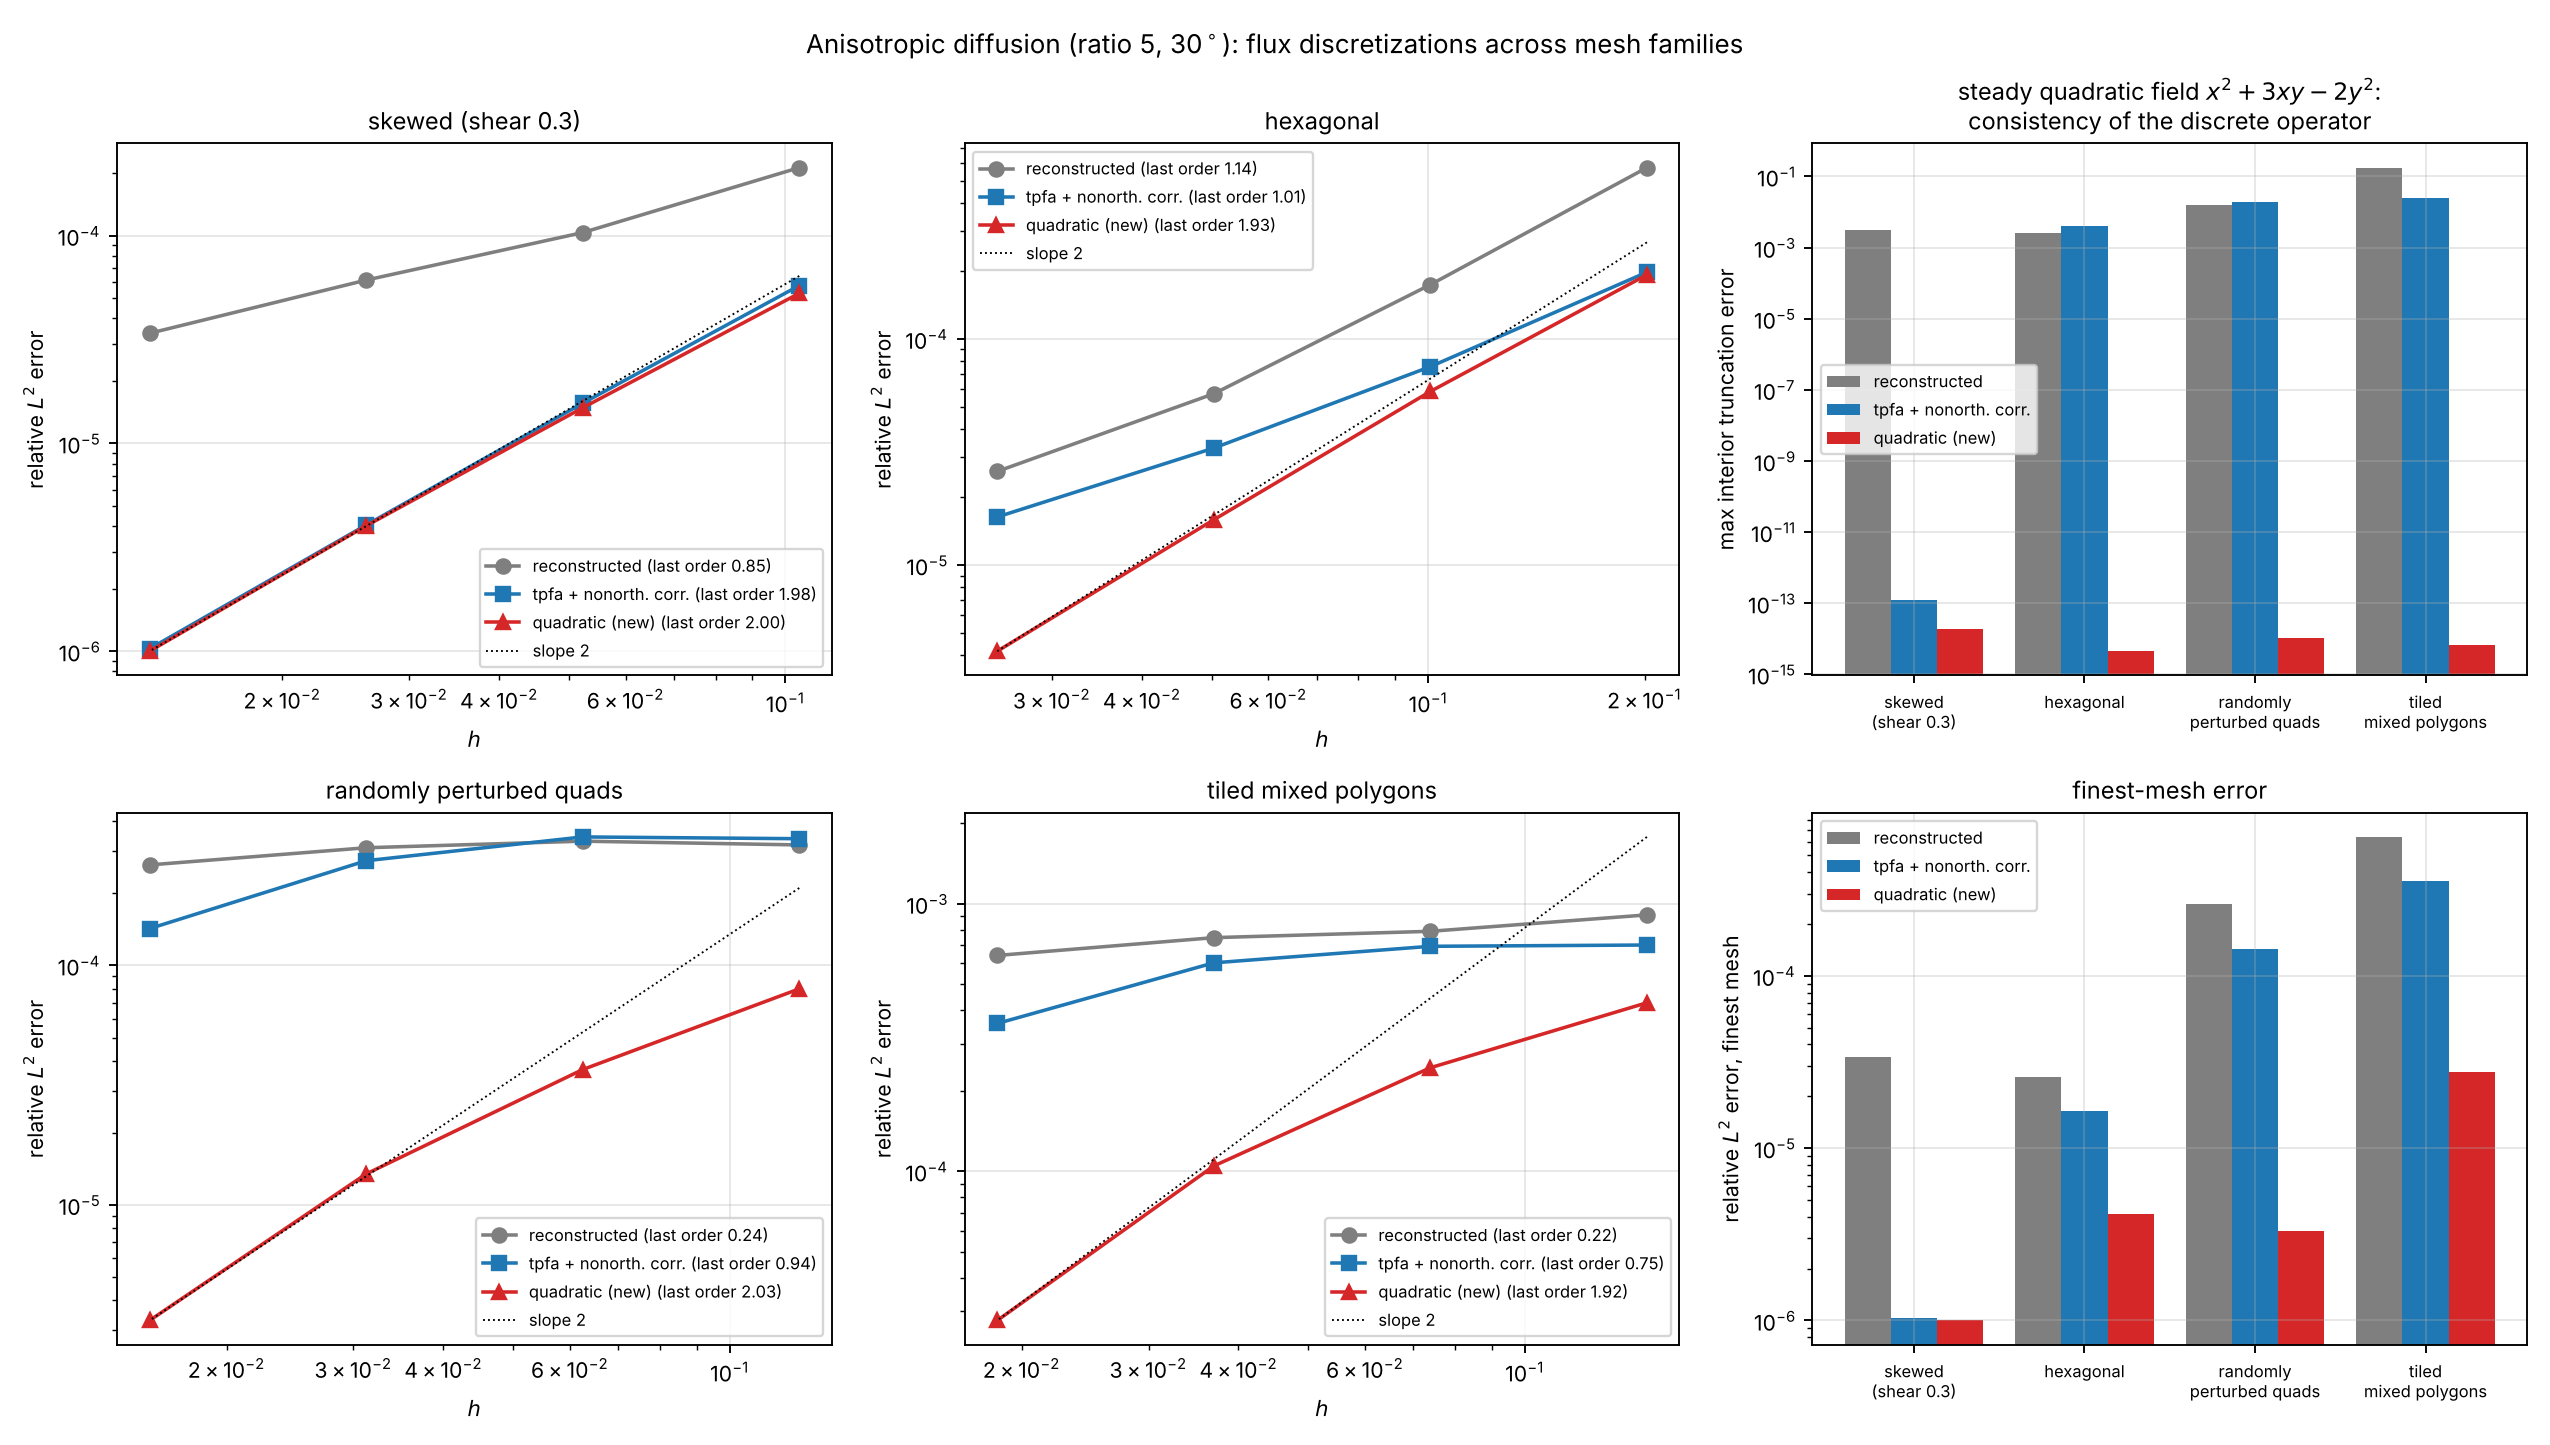
\includegraphics[width=\textwidth]{test_plots/flux_reconstruction/quadratic_flux.png}
\caption{Anisotropic diffusion (ratio 5, $30^\circ$), consistent cell-average
data, Crank--Nicolson.  Four mesh families; top right: maximum interior
truncation error of the steady operator on $x^2+3xy-2y^2$; bottom right:
finest-mesh error.}
\label{fig:Q}
\end{figure}

\begin{table}[h]
\centering
\caption{Relative $L^2$ error on the finest mesh (finest-pair observed order).
Quadratic truncation error in the last column block.}
\small
\begin{tabular}{@{}lccc|c@{}}
\toprule
mesh & reconstructed & TPFA + corr. & \textbf{quadratic} & truncation (quad.\ / TPFA) \\
\midrule
skewed ($n=128$) & $3.39\mathrm{e}{-5}\ (0.85)$ & $1.03\mathrm{e}{-6}\ (1.98)$ & $1.00\mathrm{e}{-6}\ (2.00)$ & $2\mathrm{e}{-14}$ / $1\mathrm{e}{-13}$ \\
hexagonal ($n=128$) & $2.60\mathrm{e}{-5}\ (1.14)$ & $1.63\mathrm{e}{-5}\ (1.01)$ & $4.17\mathrm{e}{-6}\ (1.93)$ & $5\mathrm{e}{-15}$ / $4\mathrm{e}{-3}$ \\
perturbed ($n=128$) & $2.63\mathrm{e}{-4}\ (0.24)$ & $1.43\mathrm{e}{-4}\ (0.94)$ & $3.29\mathrm{e}{-6}\ (2.03)$ & $1\mathrm{e}{-14}$ / $2\mathrm{e}{-2}$ \\
tiled ($n=96$) & $6.40\mathrm{e}{-4}\ (0.22)$ & $3.57\mathrm{e}{-4}\ (0.75)$ & $2.77\mathrm{e}{-5}\ (1.92)$ & $7\mathrm{e}{-15}$ / $3\mathrm{e}{-2}$ \\
\bottomrule
\end{tabular}
\label{tab:Q}
\end{table}

On the sheared mesh the corrected TPFA is already second order, because a
uniform shear keeps the face midpoint at the midpoint of the centroids and
makes its gradient correction exact for quadratics.  The quadratic flux matches
it there and is the only option that stays second order on hexagonal, randomly
perturbed and mixed polygonal meshes, with finest-mesh errors $4$--$80\times$
smaller.  The AFC limiters accept it as their high-order target
(\texttt{flux\_discretization="quadratic"}) and remain strictly bounded (unit
test).

%=============================================================================
\section{Limitations and next steps}
%=============================================================================
\begin{itemize}[leftmargin=*]
\item The envelope bounds accumulate $\Delta t\max q^\pm$ and can become loose
  for long runs; a sharper envelope would solve the source-only problem
  locally.  The relaxed local limiter is not strictly bound-preserving.
\item The reconstructed-flux audit attributes energy correctly but does not
  cure the apparent-capacity defects it reveals; the enthalpy solver does.  The
  Dirichlet-band latent jump is a modelling artefact of initial data that are
  inconsistent with the boundary data; consistent initial data or face-based
  Dirichlet conditions would remove it.
\item The quadratic flux is not provably coercive.  Numerically, the symmetric
  part of the operator is positive definite and the time-stepping spectrum lies
  in the right half plane on all four mesh families for anisotropy up to
  $10^4$ (unit tests).  It is not monotone (use it as the high-order target of
  the AFC limiters for bounds) and has $\approx21$ non-zeros per row (vs.\ 5 for
  TPFA).  Its geometry is precomputed once ($6$\,s for $16\,384$ cells) and
  re-assembly is vectorized ($0.12$\,s), which makes temperature-dependent
  (tensor) conductivity practical.  This is supported, with face temperatures
  from the quadratic reconstruction, and converges at order $\approx1.9$ on skewed
  and hexagonal meshes.  The same work found and fixed a first-order defect in
  the solver's nonlinear Crank--Nicolson step (the explicit half used
  $\mathsf A(u^{n+1})$).
\item A measured gap analysis against FiPy, scikit-fem, FEniCS and deal.II
  (2D only, Python-loop setup cost, no preconditioned or parallel solvers,
  band Dirichlet, solver-specific APIs) is in
  \path{docs/research/gap_analysis_vs_established_codes.md}.
\item The external comparison is for linear problems.  A nonlinear (Stefan)
  cross-code comparison would require writing an enthalpy model in the
  external code, which would no longer be independent.  The Neumann solution
  serves as the external reference for the nonlinear case.
\end{itemize}

\section{Reproducibility}
\begin{verbatim}
python -m pip install -r requirements-external.txt
export MPLCONFIGDIR=/tmp/matplotlib
python -m pytest tests/test_afc.py tests/test_boundary_flux.py \
       tests/test_external_codes.py tests/test_quadratic_flux.py -q
python quadratic_flux_study.py           # ~4 min
python dmp_source_study.py               # ~1 min
python direction_c_flux_audit_study.py   # ~1 min
python external_code_comparison.py       # ~3 min
\end{verbatim}
CI runs the cross-code tests in a separate job that installs the pinned
external codes from \path{requirements-external.txt}.

\begin{thebibliography}{9}
\bibitem{kuzmin2009} D.~Kuzmin, Explicit and implicit FEM-FCT algorithms with
  flux linearization, \emph{J.\ Comput.\ Phys.} 228 (2009) 2517--2534.
\bibitem{zalesak1979} S.~T. Zalesak, Fully multidimensional flux-corrected
  transport algorithms for fluids, \emph{J.\ Comput.\ Phys.} 31 (1979) 335--362.
\bibitem{zhang2010} X.~Zhang and C.-W. Shu, On maximum-principle-satisfying
  high order schemes for scalar conservation laws, \emph{J.\ Comput.\ Phys.}
  229 (2010) 3091--3120.
\bibitem{hughes2000} T.~J.~R. Hughes, G.~Engel, L.~Mazzei and M.~G. Larson,
  The continuous Galerkin method is locally conservative, \emph{J.\ Comput.\
  Phys.} 163 (2000) 467--488.
\bibitem{guyer2009} J.~E. Guyer, D.~Wheeler and J.~A. Warren, FiPy: partial
  differential equations with Python, \emph{Comput.\ Sci.\ Eng.} 11(3) (2009) 6--15.
\bibitem{gustafsson2020} T.~Gustafsson and G.~D. McBain, scikit-fem: a Python
  package for finite element assembly, \emph{J.\ Open Source Softw.} 5(52)
  (2020) 2369.
\bibitem{carslaw1959} H.~S. Carslaw and J.~C. Jaeger, \emph{Conduction of Heat
  in Solids}, 2nd ed., Oxford University Press, 1959.
\end{thebibliography}

\end{document}
